In this chapter, we describe the dataset, the dMRI acquisition and preprocessing steps, and brain mask extraction. We then outline the FBA pipeline with LoRE-SD–specific steps, highlight key parameters, and describe the statistical analysis, including strategies to increase statistical power by reducing the number of fixels.

\section{Dataset Description}
The dataset consists of 101 women divided into three groups: two breast cancer groups and one healthy control (HC) group. The first breast cancer group includes patients undergoing chemotherapy (CP), while the second group includes cancer patients not receiving chemotherapy (CM). Data were collected three months post-chemotherapy.

The principal characteristics of the subjects belonging to the three groups are described in \cref{tab:dataset}.

\begin{table}[H]
    \caption*{\textbf{Subject characteristics by group}} % visible bold title
    \centering 
    \begin{tabular}{|p{6em} c c|} % wider first column
    \hline
    \rowcolor{bluepoli!40} % comment this to remove the color
    \textbf{Group} & \textbf{Number of Subjects} & \textbf{Mean Age (SD)} \T\B \\
    \hline \hline
    CP & 28 & 50.36 (8.61) \T\B \\
    CM & 32 & 51.93 (7.15) \T\B \\
    HC & 41 & 47.46 (10.29) \B \\
    \hline
    \end{tabular}
    \\[10pt]
    \caption{Mean and standard deviation (SD) of age per group are indicated.}
    \label{tab:dataset}
\end{table}

\section{Acquisition Protocol}
Diffusion-weighted imaging data were acquired using a Philips Achieva 3T MRI scanner with a Spin Echo sequence. The data consists of 157 volumes, including multiple b-values (0, 500, 1200, 2400, 4000), corresponding to a multi-shell DWI acquisition. Repetition Time was 6.4 seconds and Echo Time was 85 ms. The number of directions for each shell is reported in \cref{tab:directions}.

\begin{table}[H]
    \caption*{\textbf{Number of gradient directions per shell}} % visible bold title
    \centering 
    \begin{tabular}{|c c|}
    \hline
    \rowcolor{bluepoli!40} % header color
    \textbf{b-value [$s/mm^2$]} & \textbf{Number of Directions} \T\B \\
    \hline \hline
    0 & 5 \T\B \\
    500 & 20 \T\B \\
    1200 & 30 \T\B \\
    2400 & 41 \T\B \\
    4000 & 61 \B \\
    \hline
    \end{tabular}
    \\[10pt]
    \caption{Number of gradient directions per shell.}
    \label{tab:directions}
\end{table}

\section{Preprocessing}
All preprocessing was performed using MRtrix3 \cite{Tournier2019}, with integration of FSL tools where noted \cite{Smith2004}.
The data underwent the following preprocessing steps:

\begin{enumerate}
    \item \textbf{Denoising:} \texttt{dwidenoise} was applied to the DWI data to reduce thermal noise using the Marchenko-Pastur principal component analysis method \cite{Veraart2016a,Veraart2016b,Cordero-Grande2019}.
    
    \item \textbf{Gibbs Ringing Removal:} \texttt{mrdegibbs} was used to suppress Gibbs ringing artifacts, improving image quality \cite{Kellner2016}.
    
    \item \textbf{Distortion and Motion Correction:} \texttt{dwifslpreproc} was employed to correct for motion, eddy-current distortions and susceptibility-induced distortions, using FSL's \texttt{eddy} tool \cite{Andersson2016}.
    
    \item \textbf{Bias Field Correction:} \texttt{dwibiascorrect} was used to correct for low frequency intensity inhomogeneities (bias field) \cite{Tustison2010}.
    
    \item \textbf{Cropping and Padding:} \texttt{mrgrid} was applied to crop and pad the image volumes, standardizing their dimensions.
    
    \item \textbf{Resampling:} The data were resampled to an isotropic voxel size of 1.3 mm using \texttt{mrgrid -regrid}.
\end{enumerate}

\section{Brain mask extraction}
\label{sec:mask}
Accurate brain masks are essential to restrict the analysis to voxels within the brain, excluding noise from surrounding non-brain tissues. This improves data quality and prevents artifacts, especially during registration, where excluding the skull allows to focus only on relevant anatomical structures, increasing the accuracy \cite{ou2014}.

We computed brain masks using two approaches:
\begin{enumerate}

    \item \textbf{SynthStrip:} SynthStrip \cite{hoopes2022} is a deep learning method that uses a convolutional neural network (CNN) trained exclusively on synthetic data. This training dataset spans a wide range of anatomies, image contrasts, and artifacts, including extreme unrealistic cases, improving the generalization ability of the model.

    \item \textbf{Tissue volume fractions:} Brain masks were generated using approximated tissue volume fraction maps estimated with MT-CSD. Specifically, the sum of the first SH coefficients ($l=0$) from the normalized WM, GM and CSF ODFs was computed for each voxel. Voxels with a total sum greater than 0.1 were included in the brain mask, assuming that brain voxels should contain non-negligible contributions from these three tissue types.
\end{enumerate}
For MT-CSD analysis, we decided to use the SynthStrip masks, while for LoRE-SD the second mask was the better approach as it excluded all noisy non brain voxels that could introduce distortion during registration. A visual comparison of the masks is shown in Figure~\ref{fig:mask}.

\begin{figure}[h]
  \centering
  \makebox[\textwidth][c]{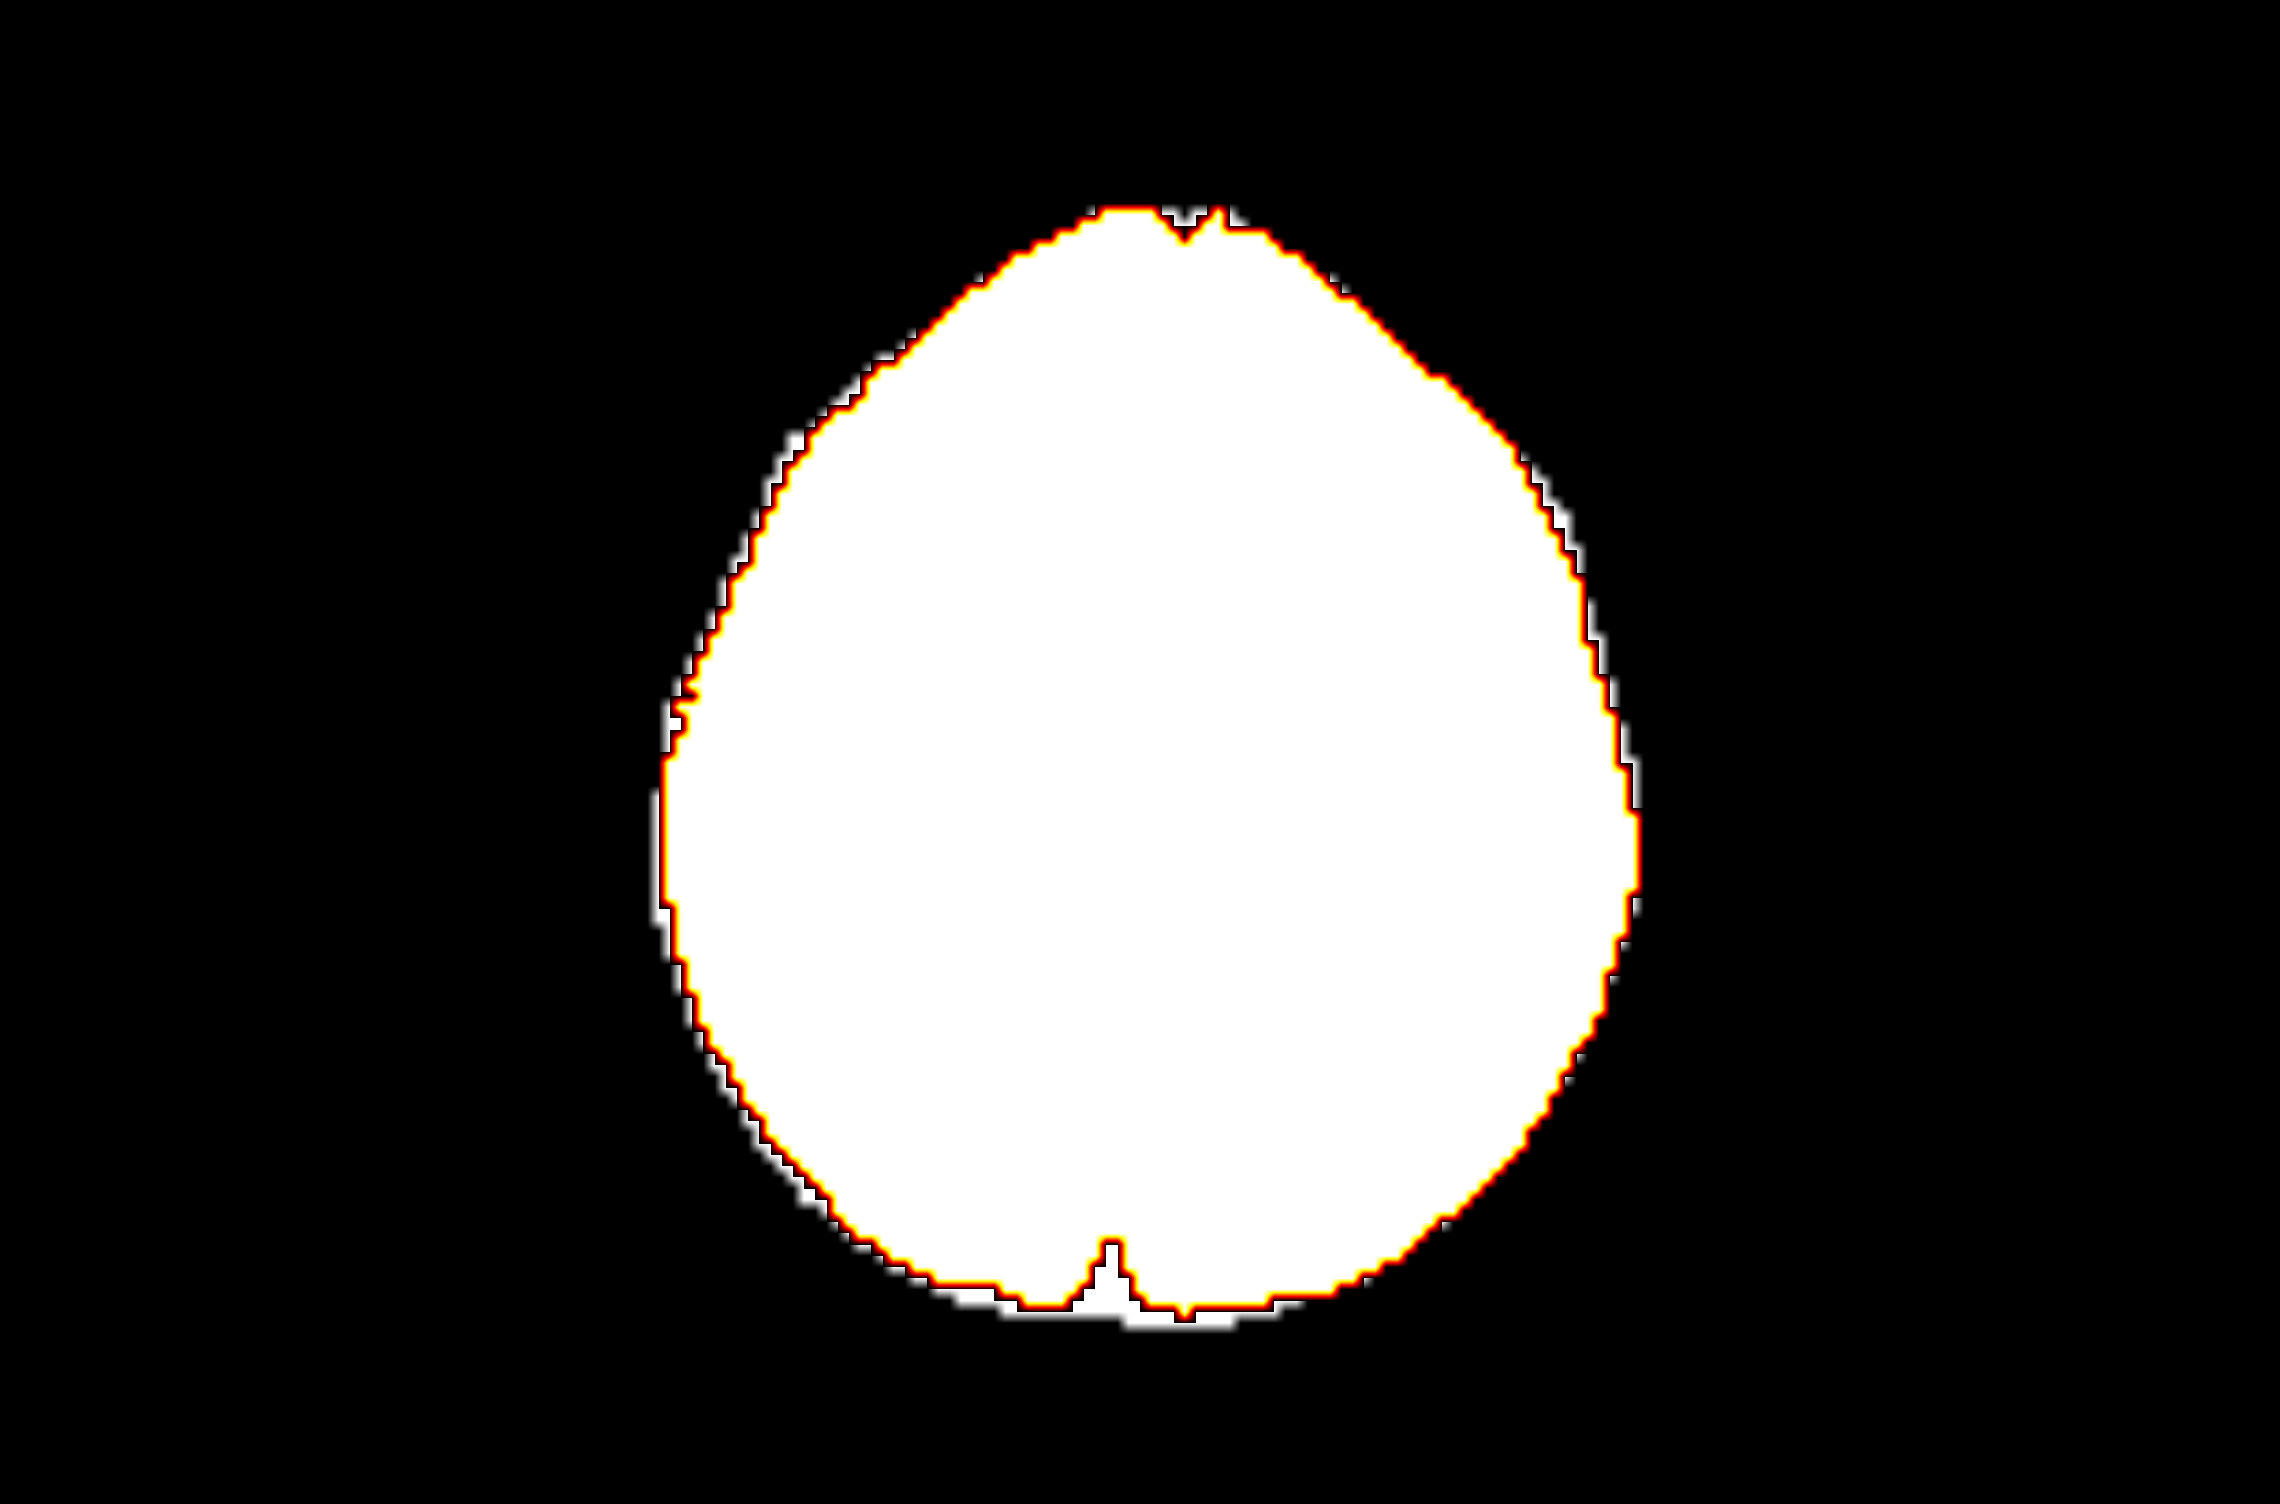
\includegraphics[width=0.6\textwidth]{Images/mask.png}}
  \caption{Example of the mask estimated using tissue volume fractions overlaid on the SynthStrip mask.}
  \label{fig:mask}
\end{figure}

\section{Analysis Pipeline}

The analysis was performed using MRtrix3 \cite{Tournier2019}. The main steps for the MT-CSD pipeline are outlined below:

\begin{enumerate}
    \item \textbf{Response Function Estimation:} Unsupervised estimation of response functions for WM, GM, and CSF was performed for each subject with \texttt{dwi2response} \cite{raffelt2019}. The estimated functions were then averaged across subjects to generate study-specific response functions for each tissue type.

    \item \textbf{MT-CSD:} Multi-tissue CSD was performed to compute WM ODFs with \texttt{dwi2fod}\cite{Jeurissen2014}.

    \item \textbf{Intensity Normalization:} \texttt{mtnormalise} was used on the ODFs to normalize them and correct for intensity bias \cite{Dhollander21}.

    \item \textbf{Template Creation:} A subset of 10 subjects per group was randomly selected for unbiased population template creation using \texttt{population\_template}. Initial alignment was performed using rigid and affine registration, followed by non-linear registration for final template optimization.

    \item \textbf{Registration to Template:} Subject ODFs were registered to the template using \texttt{mrregister}. This included affine and non-linear ODF-guided registration and reorientation \cite{Raffelt12}. The registration is symmetric, computing forward (subject~$\rightarrow$~template) and inverse (template~$\rightarrow$~subject) warps by aligning both images in a midway space.

    \item \textbf{Template Mask Generation:} The group analysis mask was defined as the intersection of all individual warped brain masks, obtained by taking the voxel-wise minimum across subjects.

    \item \textbf{Remove Cerebellum and Brainstem:} These regions were excluded to focus on the rest of the brain, thereby increasing statistical power by reducing the number of comparisons and speeding up the analysis.

    \item \textbf{Fixel Mask Generation:} ODFs were segmented in the template to create a fixel analysis mask using \texttt{fod2fixel}.

    \item \textbf{Warp Subject ODFs:} Each subject's ODFs were warped to the template space without reorientation using  \texttt{mrtransform}.

    \item \textbf{AFD Computation:} AFD values were computed by segmenting each subject's warped ODFs in the template space.

    \item \textbf{Fixel Reorientation:} Fixels were reoriented based on local angular transformations derived from the deformation fields at each voxel with \texttt{fixelreorient}.

    \item \textbf{Fixel Correspondence:} Fixels from each subject were matched to the template fixels using an angular threshold to identify the closest correspondence with minimal angular difference with \texttt{fixelcorrespondence}.

    \item \textbf{FC and FDC Computation:} Fixel-wise FC values were found from the Jacobian of the warp fields using \texttt{warp2metric}, log-transformed to ensure data are centred around zero and normally distributed, and multiplied by AFD to compute FDC.

    \item \textbf{Tractography and Smoothing:} A whole-brain tractogram was generated starting from the template, followed by the generation of the connectivity matrix and fixel-wise smoothing (\texttt{tckgen, fixelconnectivity, fixelfilter}).

    \item \textbf{Statistical Analysis:} Group-wise statistical comparisons were conducted using \texttt{fixelcfestats}, which implements a GLM and CFE, by defining appropriate design and contrast matrices.
\end{enumerate}

In the case of LoRE-SD, the pipeline does not include steps 1-3. The alternative steps are as follows:

\begin{enumerate}
    \item  \textbf{LoRE-SD: } LoRE-SD is applied to the diffusion data to obtain for each subject in each voxel a local response function and a unit-normalized ODF. The response function is described as a linear combination of Gaussian basis functions with corresponding weights (Gaussian fractions).

    \item \textbf{Contrasts Computation:} Contrast matrices are defined either assigning values to the grid of axial and radial diffusivities or by finding them through least squares from a pre-existing contrast. For each subject contrast images are obtained by taking the inner product of the contrast matrix with the Gaussian fractions found through LoRE-SD.

    \item \textbf{ODFs Scaling:} Unit-normalized ODFs found with LoRE-SD are scaled by performing a voxel-wise multiplication with the contrasts found in the previous step.

    \item \textbf{Cropping:} To completely exclude noisy ODFs from the analysis, images are cropped using brain masks, by multiplying the ODFs by the binary mask. This way, everything outside the brain is set to zero.
    
\end{enumerate}

\section{Contrast Computation in LoRE-SD}
Contrast matrices are defined by assigning weigths from 0 to 1 to the Gaussian basis functions parametrized by $\lambda_{\parallel}$ and $\lambda_{\perp}$.
Figure~\ref{fig:contrast} shows how the intra-axonal contrast is obtained in a 10 by 10 grid of basis functions. The contrast can be modified by adjusting the rate of the exponential decay of the weights with increasing $\lambda_{\perp}$, or by imposing anisotropy, meaning that all cells on the diagonal are set to 0, suppressing all isotropic basis functions.

Another contrast mimics the value of FA and it can be seen in Figure~\ref{fig:fa}. The equation of the FA metric from DTI (\ref{eq:FA}), with $\lambda_{\parallel}$ as $\lambda_{1}$ and $\lambda_{\perp}$ as $\lambda_{2}$ and $\lambda_{3}$, is used to assign a value to each combination of parameters.

\begin{figure}[h]
  \centering
  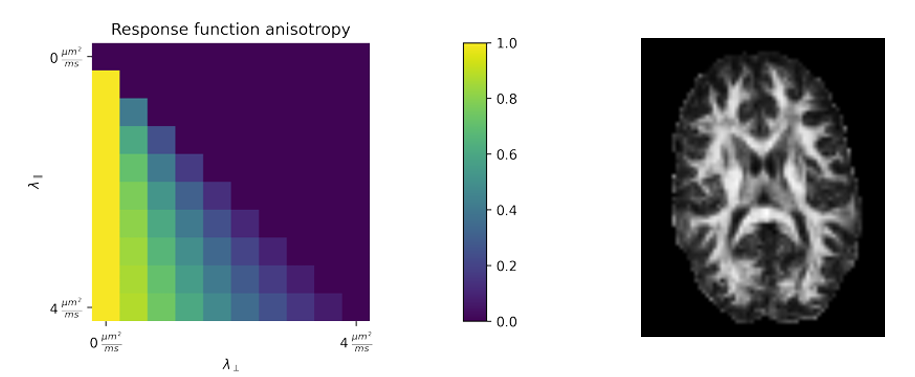
\includegraphics[width=0.7\textwidth]{Images/fa.png} % or use height= for vertical sizing
  \caption{Contrast matrix defining the FA contrast and resulting contrast for a subject.}
  \label{fig:fa}
\end{figure}
 

In theory, any contrast can be used to directly scale the ODFs. Another approach is to derive contrast matrices from existing contrast images by solving an optimization problem. A least-squares optimization can be used to determine the combination of basis functions (contrast matrix) that best reproduces the input contrast when applied to the Gaussian fractions from LoRE-SD. The problem can be written as a constrained linear least square problem:

\begin{align}
\min_{\boldsymbol{x}} \quad & \frac{1}{2} \left\| A \boldsymbol{x} - \boldsymbol{b} \right\|^2 \\
\text{subject to} \quad & \boldsymbol{0} \leq \boldsymbol{x} \leq \boldsymbol{1}
\end{align}
Here, $A$ contains the input Gaussian fractions that define the local response function in each voxel, b is the target image contrast assigning a value to each voxel, and $\boldsymbol{x}$ represents the weights for each Gaussian basis function (each point on the grid). We impose that the weights have to be between 0 and 1. The optimization problem was solved using the \texttt{lsq\_linear} function from the SciPy library \cite{Virtanen2020}.
Solving this provides a data-driven contrast matrix that emphasizes the contribution of the tissue compartments underlying the given image contrast. This approach not only provides a means to scale the ODFs, but also offers insight into the characteristics of the contrast.
\\A possible meaningful contrast to replicate is the WM volume fractions estimated from MT-CSD. Specifically, the first SH coefficient of the WM ODF can be used as the target contrast $\boldsymbol{b}$.

\section{Removal of Cerebellum and Brainstem}
To improve statistical power and reduce computational load, the cerebellum and brainstem were excluded from the FBA. The segmentation was performed using the T1-weighted anatomical images of the subjects, following these steps:

\begin{enumerate}
    \item \textbf{Rigid Registration:} The average $b=0$ diffusion image was rigidly registered to the subject's T1-weighted image. Rigid registration is used because the images belong to the same subject so the difference won't be in the anatomy but only due to the patient moving or different positioning. 

    \item \textbf{Transform T1 to DWI Space:} The inverse of the above transformation was applied to bring the T1-weighted image into diffusion space.

    \item \textbf{Transform to Template Space:} The subject-specific non-linear warp (obtained during registration to the group template) was then used to bring the T1 image from diffusion space to template space.

    \item \textbf{Segmentation of Cerebellum and Brainstem:} SynthSeg \cite{billot2023} was used to segment the cerebellum and brainstem from the T1-weigted image in template space. SynthSeg is a deep learning-based tool that uses CNNs trained entirely on synthetic data, enabling robust segmentation without the need for retraining or fine-tuning. This resulted in a binary mask for each subject that excludes the cerebellum and brainstem.

    \item \textbf{Mask Averaging:} The individual binary masks were averaged across subjects. Voxels with an average value below 0.5 were set to 0, removing only voxels consistently excluded across subjects.

    \item \textbf{Resolution Adjustment:} The resulting mask, originally at T1 resolution, was downsampled to match the resolution of the diffusion data.

    \item \textbf{Combination with Template Mask:} The cerebellum-brainstem exclusion mask was combined with the main template mask using a voxel-wise minimum (logical AND), ensuring that only voxels common to all subjects and excluding unwanted regions were included in the analysis.

    \item \textbf{Fixel Mask Creation:} The final voxel-wise mask was converted to a fixel-wise mask by assigning a value of 0 to all fixels in voxels with value 0, and 1 to the rest using MRtrix3 command \texttt{voxel2fixel} \cite{Tournier2019}. This fixel mask was used to define the region of interest in the statistical analysis.
\end{enumerate}

\section{Fixels Extraction}
\label{sec:extract}

\begin{table}[H]
    \caption*{\textbf{Number of fixels obtained by changing the threshold for different ODF templates}} % bold visible title
    \centering 
    \begin{tabular}{|l c c|}
    \hline
    \rowcolor{bluepoli!40}
    \textbf{ODF Template} & \textbf{Threshold} & \textbf{Number of fixels} \T\B \\
    \hline \hline
    MT-CSD & 0.06 & 365585 \T\B \\
    LoRE-SD with intra-axonal scaling & 0.06 & 379857 \T\B \\
    LoRE-SD with intra-axonal scaling & 0.07 & 327759 \T\B \\
    LoRE-SD with FA scaling & 0.06 & 455263 \T\B \\
    LoRE-SD with FA scaling & 0.07 & 379065 \T\B \\
    LoRE-SD with FA scaling & 0.08 & 323570 \B \\
    \hline
    \end{tabular}
    \\[10pt]
    \caption{Number of fixels obtained by changing the threshold value on the lobe amplitude for different ODF templates.}
    \label{tab:fixels}
\end{table}


To derive fixels from both the template and subject ODFs, a threshold on the lobe amplitude must be defined. This threshold determines which peaks in the ODFs are segmented as fixels. It is important to extract a sufficiently large number of fixels and to ensure that fixels are present also in regions with crossing fibres. The optimal threshold may vary based on the data and the preprocessing steps. Also it can depend on whether MT-CSD or LoRE-SD is used, and for the latter also on which contrast was used for scaling. The thresholds and the resulting numbers of fixels can be found in \cref{tab:fixels}. 

Figure~\ref{fig:fixels} shows some details of the extracted fixels.

\begin{figure}[H]
  \centering
  \subfloat[MT-CSD ($\tau = 0.06$)\label{fig:mtcsd}]{
    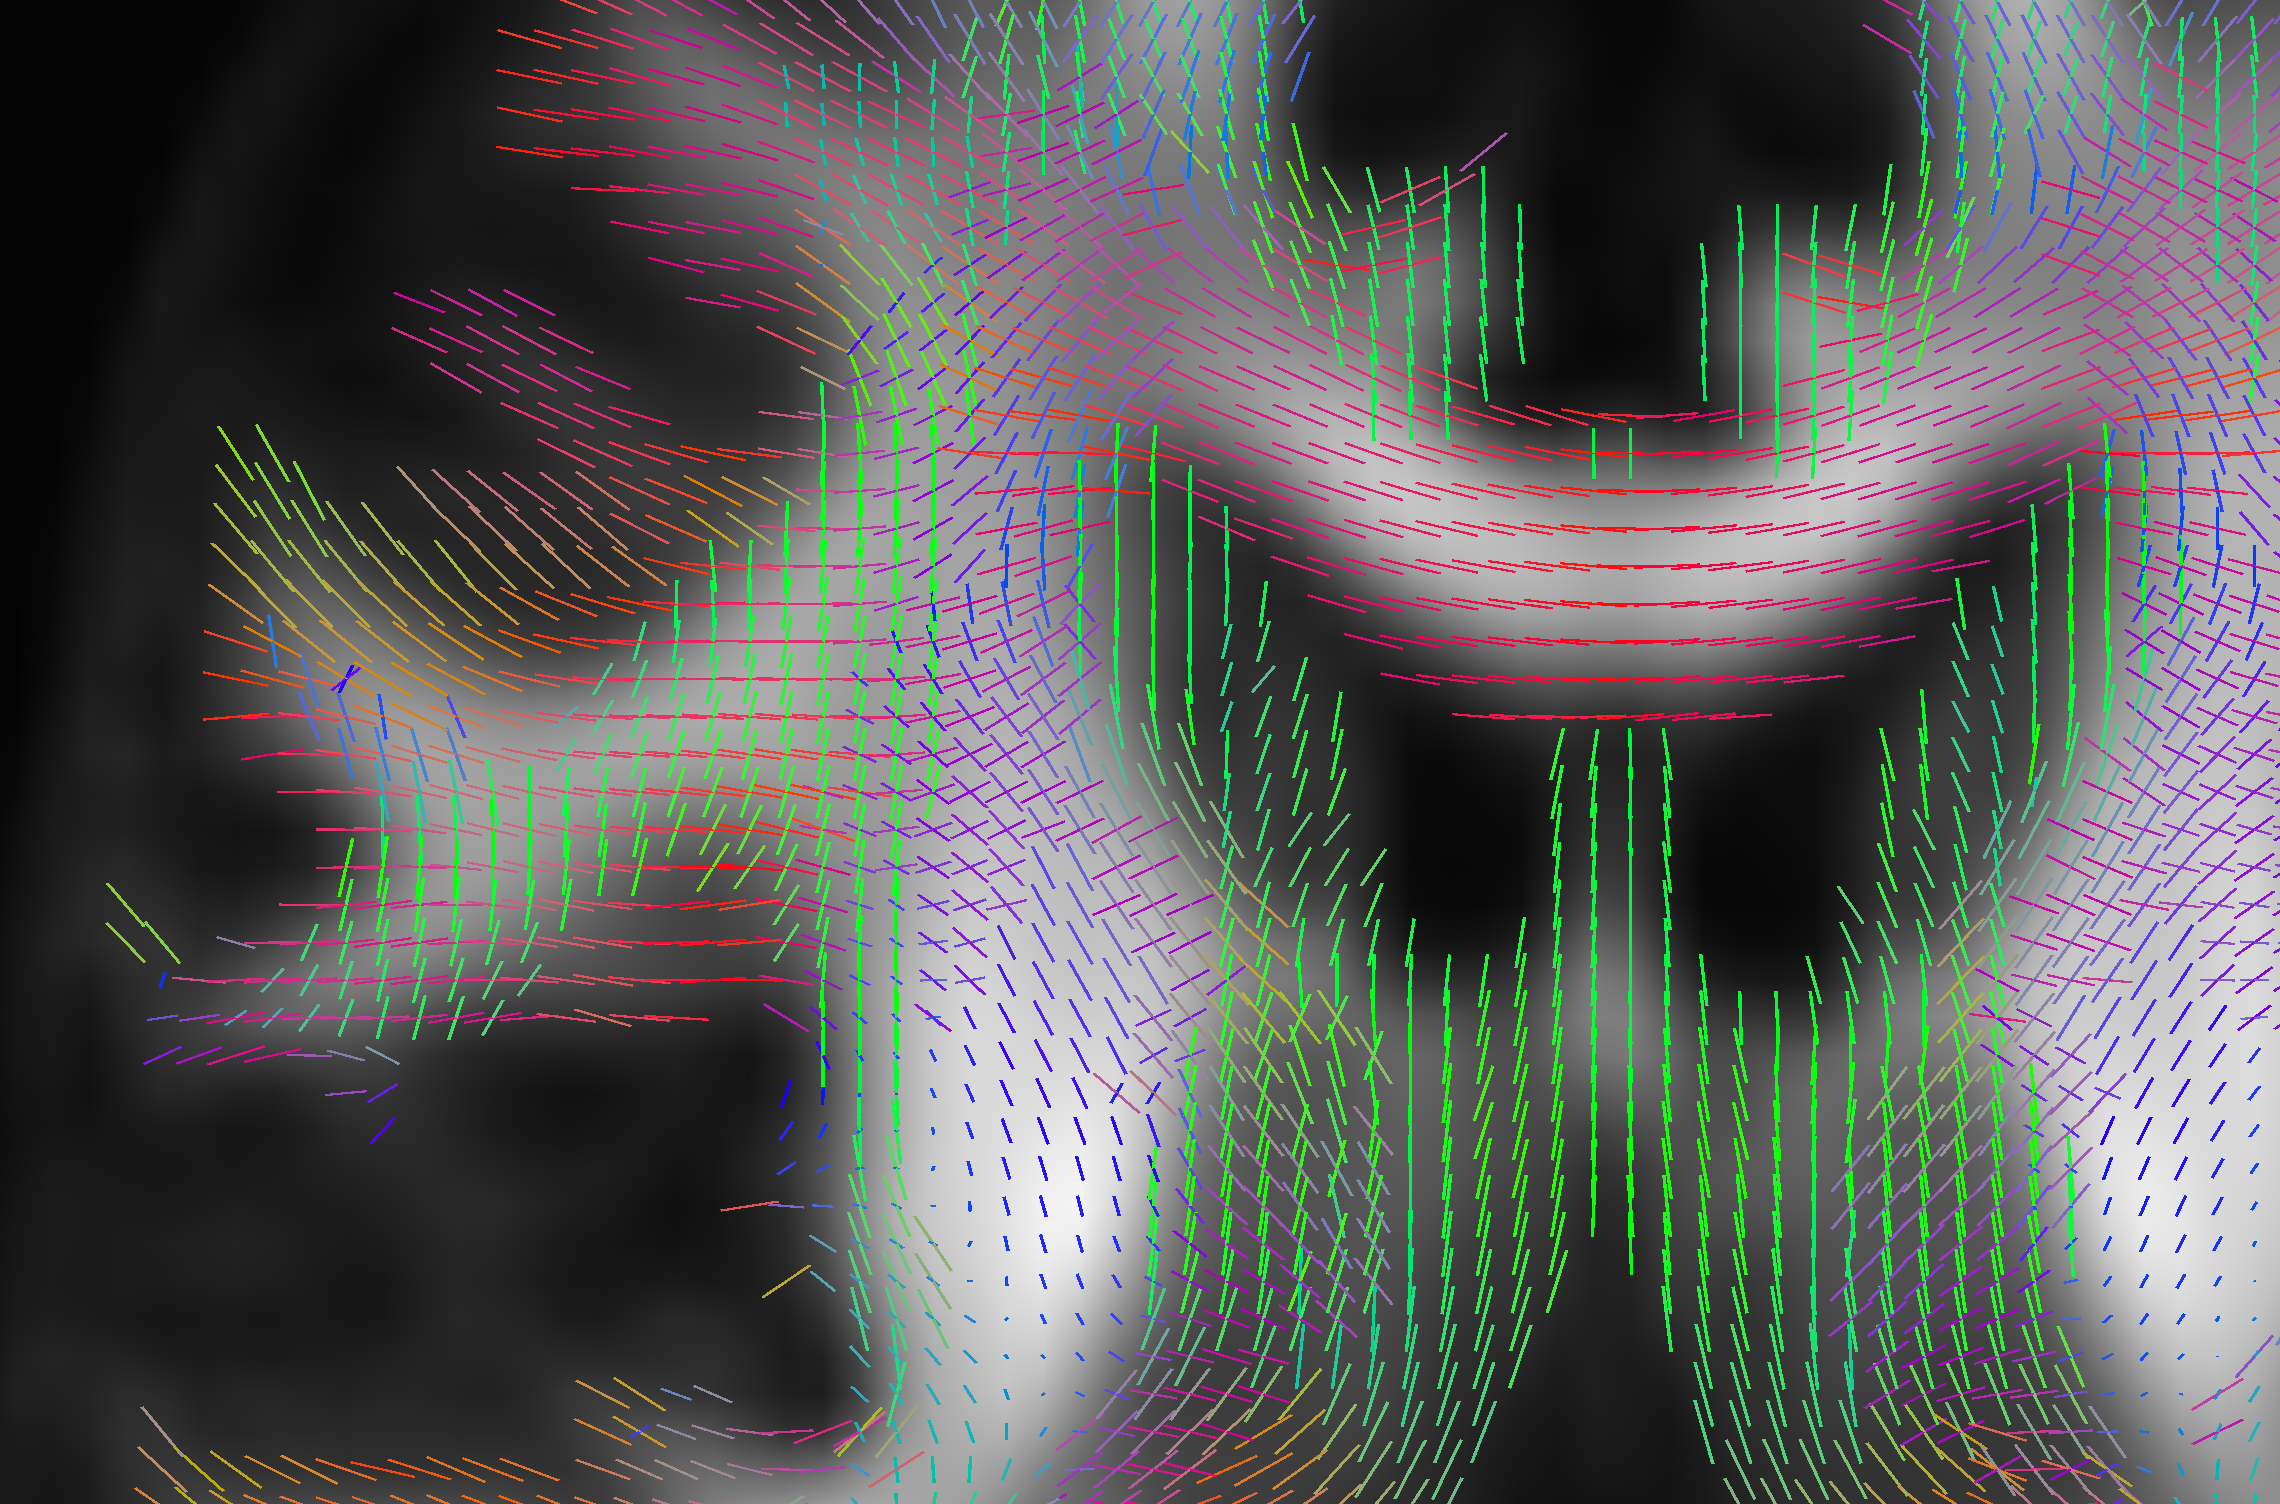
\includegraphics[width=0.45\textwidth]{Images/comparison_MTCSD0005.jpg}
  }
  \hfill
  \subfloat[LoRE-SD (intra-axonal, $\tau = 0.06$)\label{fig:lore06}]{
    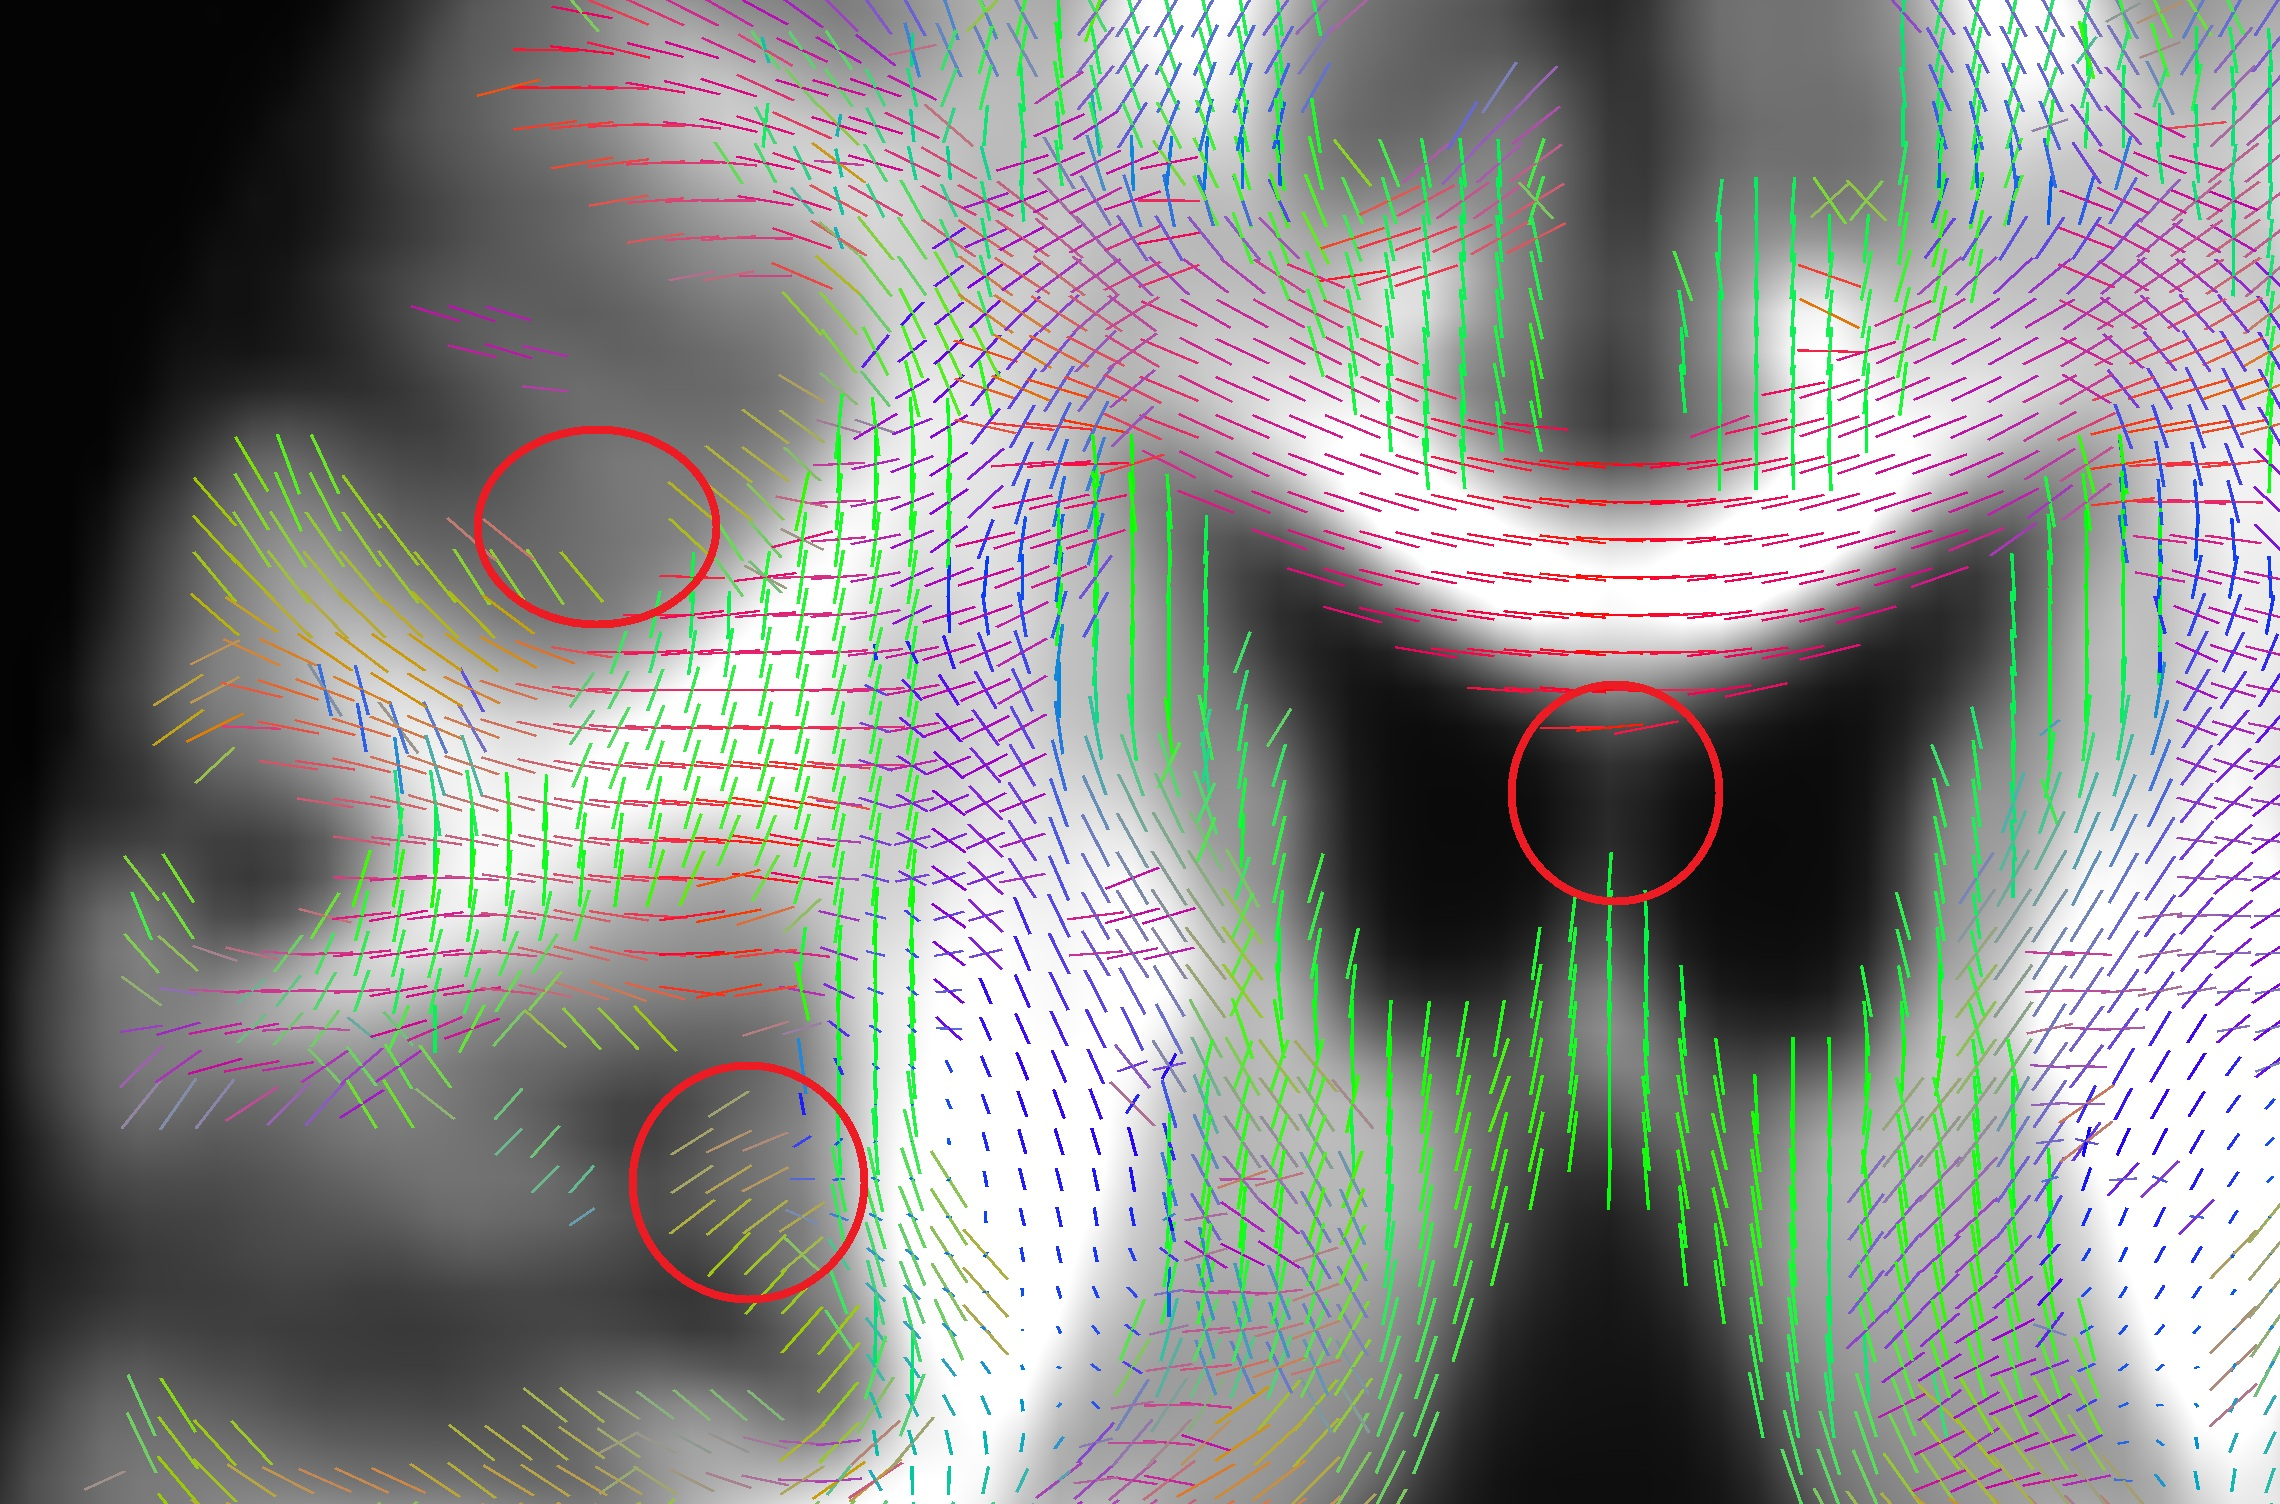
\includegraphics[width=0.45\textwidth]{Images/comparison_intra_axona_annotated.jpg}
  }
  \hfill
  \subfloat[LoRE-SD (intra-axonal, $\tau = 0.07$)\label{fig:lore07}]{
    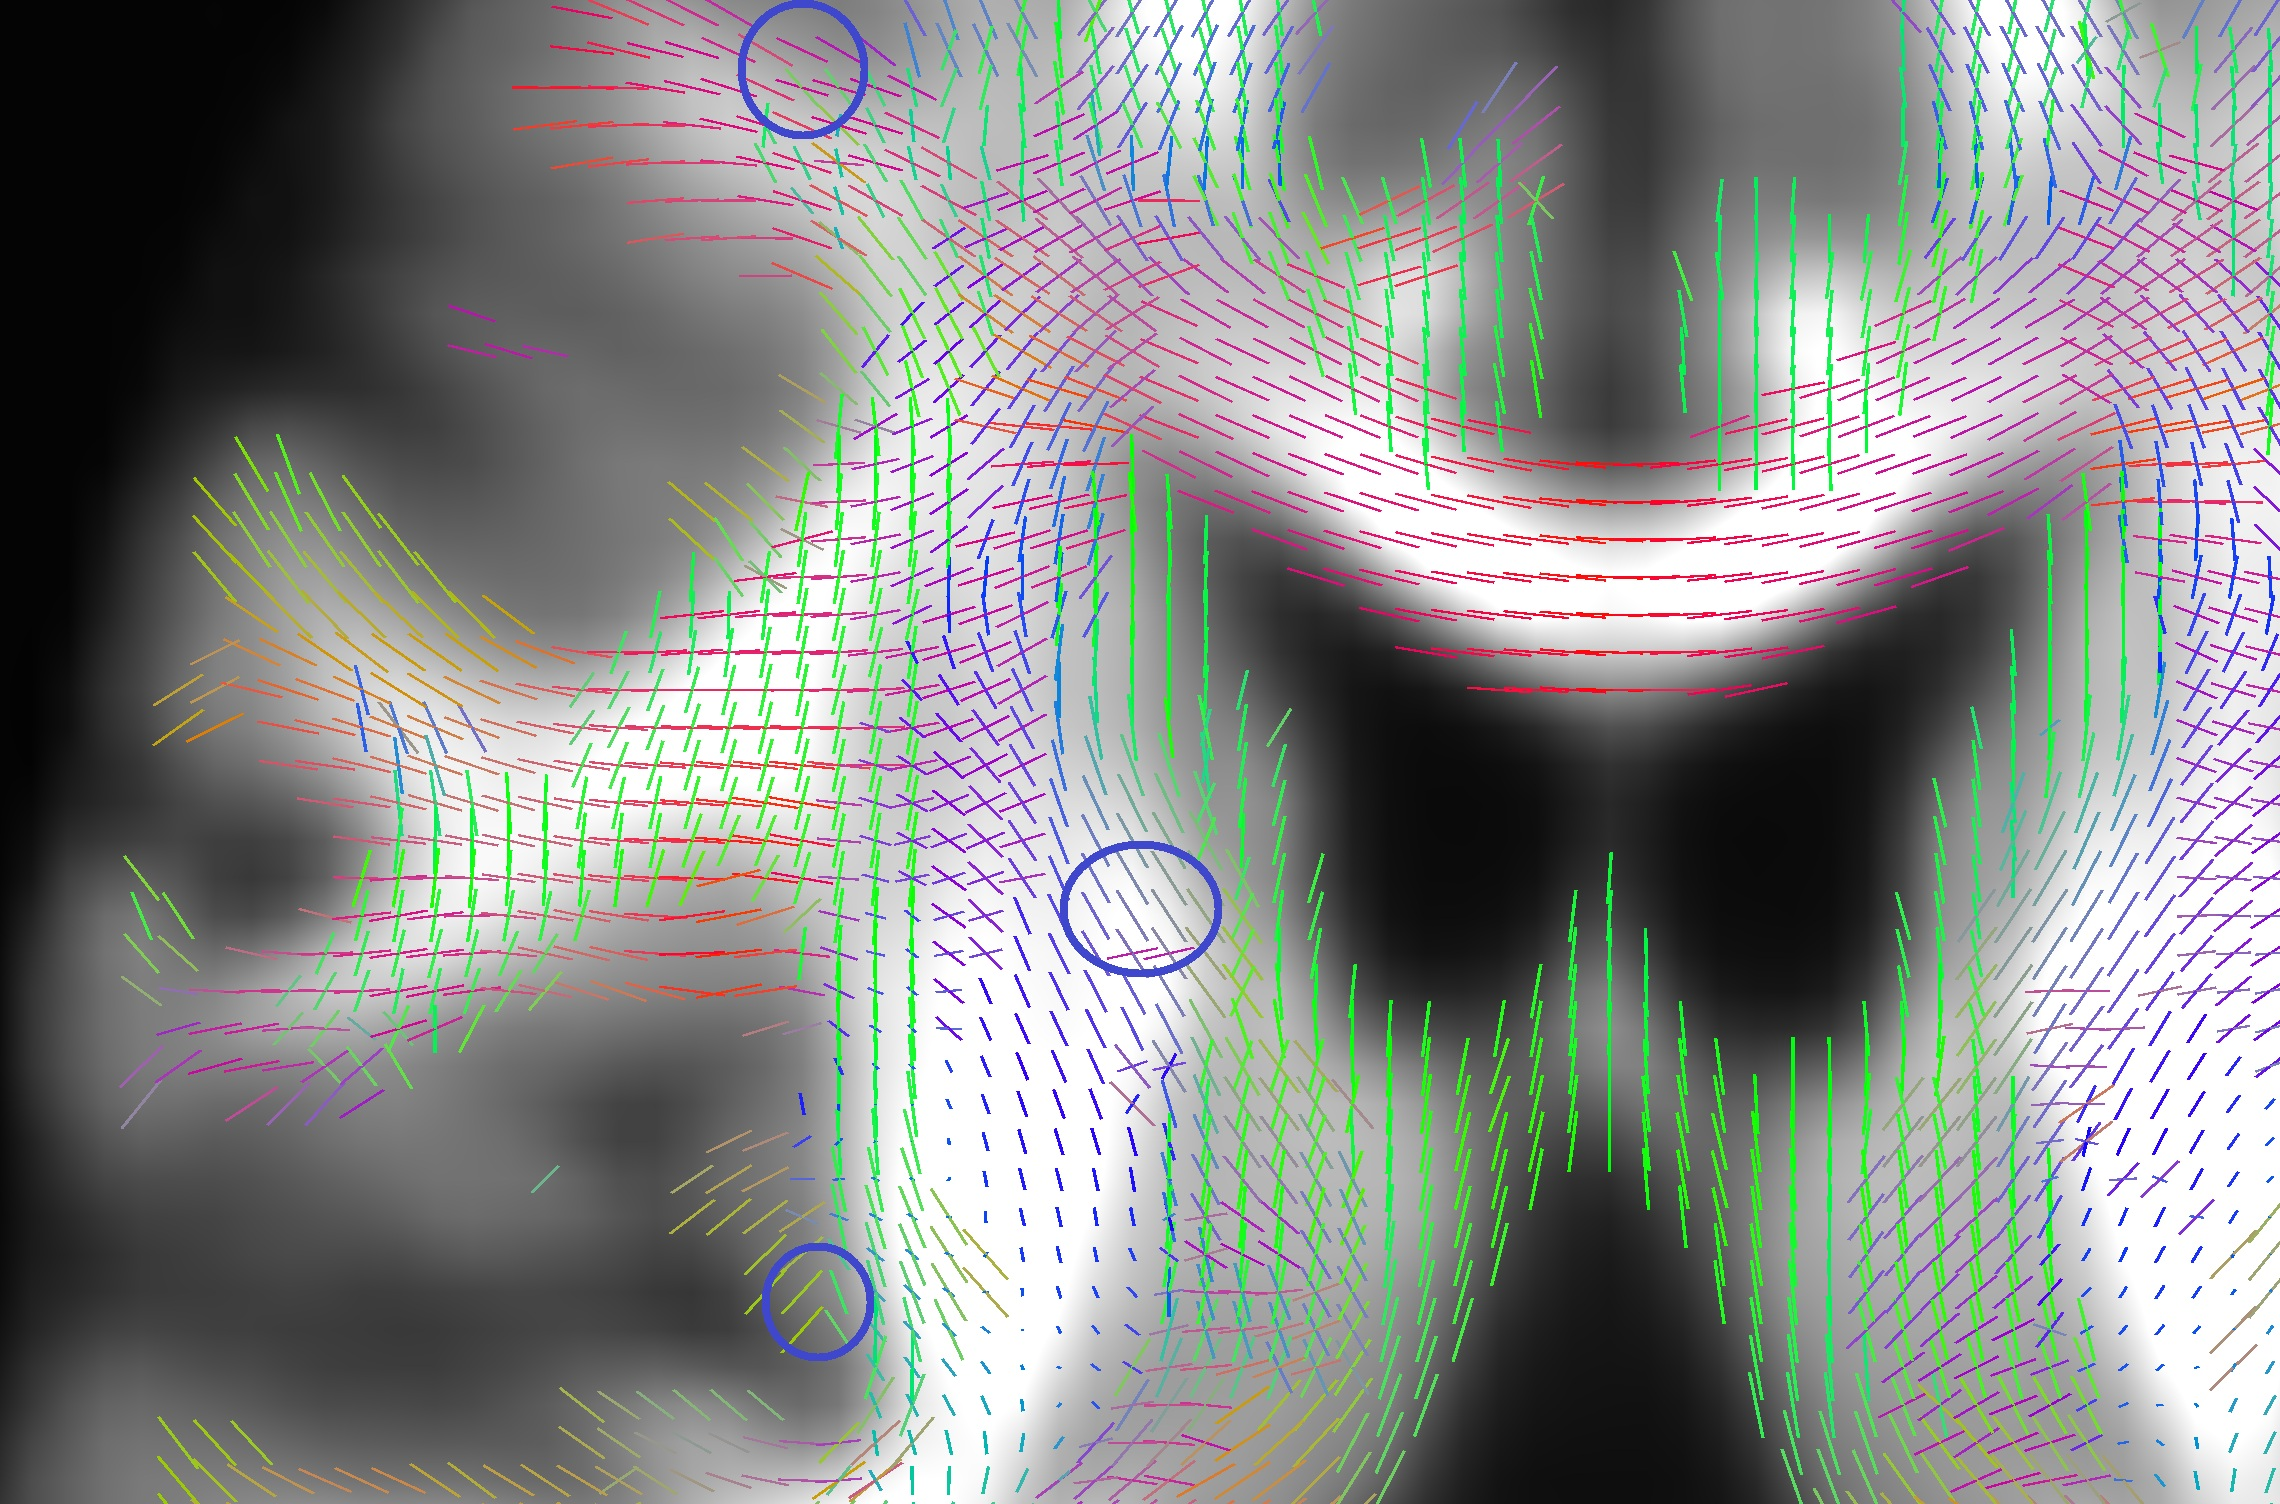
\includegraphics[width=0.45\textwidth]{Images/comparison_intra_axonal_less_annotated.jpg}
  }
  \caption[Fixel masks]{Fixel masks for the first 3 cases reported in \cref{tab:fixels}. $\tau$ indicates the threshold on the lobe amplitude of the ODFs. Red circles show regions where MT-CSD and LoRE-SD differ. Blue circles show regions where fixels are lost when increasing the threshold.}
  \label{fig:fixels}
\end{figure}



It can be noted that there are some differences in the fixels extracted with the two methods. With the same threshold LoRE-SD results in a higher number of fixels, but increasing the threshold could lead to the loss of some important fixels. Figure~\ref{fig:fixels} shows that increasing the threshold leads to the loss of some fixels in crossing fiber regions. For this reason the lower threshold was chosen for the intra-axonal contrast. For the FA contrast 0.07 seems to be a better choice.


\section{Tractography}
The tractography algorithm employed was iFOD2 \cite{Tournier2010}, a probabilistic method that starts from the information contained in the ODFs. The algorithm favors tracking along directions with higher ODF amplitudes, while still allowing propagation through lower-amplitude directions as long as values are higher than a given threshold. iFOD2 generates streamlines by propagating along short arcs tangent to the current direction, which improves anatomical plausibility. Tracking was seeded randomly within the brain mask. The minimum ODF amplitude required to continue tracking was set to 0.06, only streamlines between 10 mm and 250 mm in length were accepted, and the maximum change in underlying fibre orientation between the start and end points of each step was set to 22.5$^\circ$. This last parameter controls the smoothness of the resulting streamlines \cite{Smith2012}. A total of 20 million streamlines were generated.

To reduce biases in tractogram density and improve biological plausibility, SIFT (Spherical-deconvolution Informed Filtering of Tractograms) was applied \cite{Smith2013}. This method refines the tractogram by iteratively removing streamlines (from 20 to 2 million in our case) to only keep the ones that best match the underlying ODFs. SIFT works by comparing the density of streamlines in each voxel with the integral of the ODF lobes in corresponding directions. The assumption is that larger ODF lobes represent regions with more axons oriented in that direction, and so with a higher density of streamlines.

\begin{figure}[h]
  \centering
  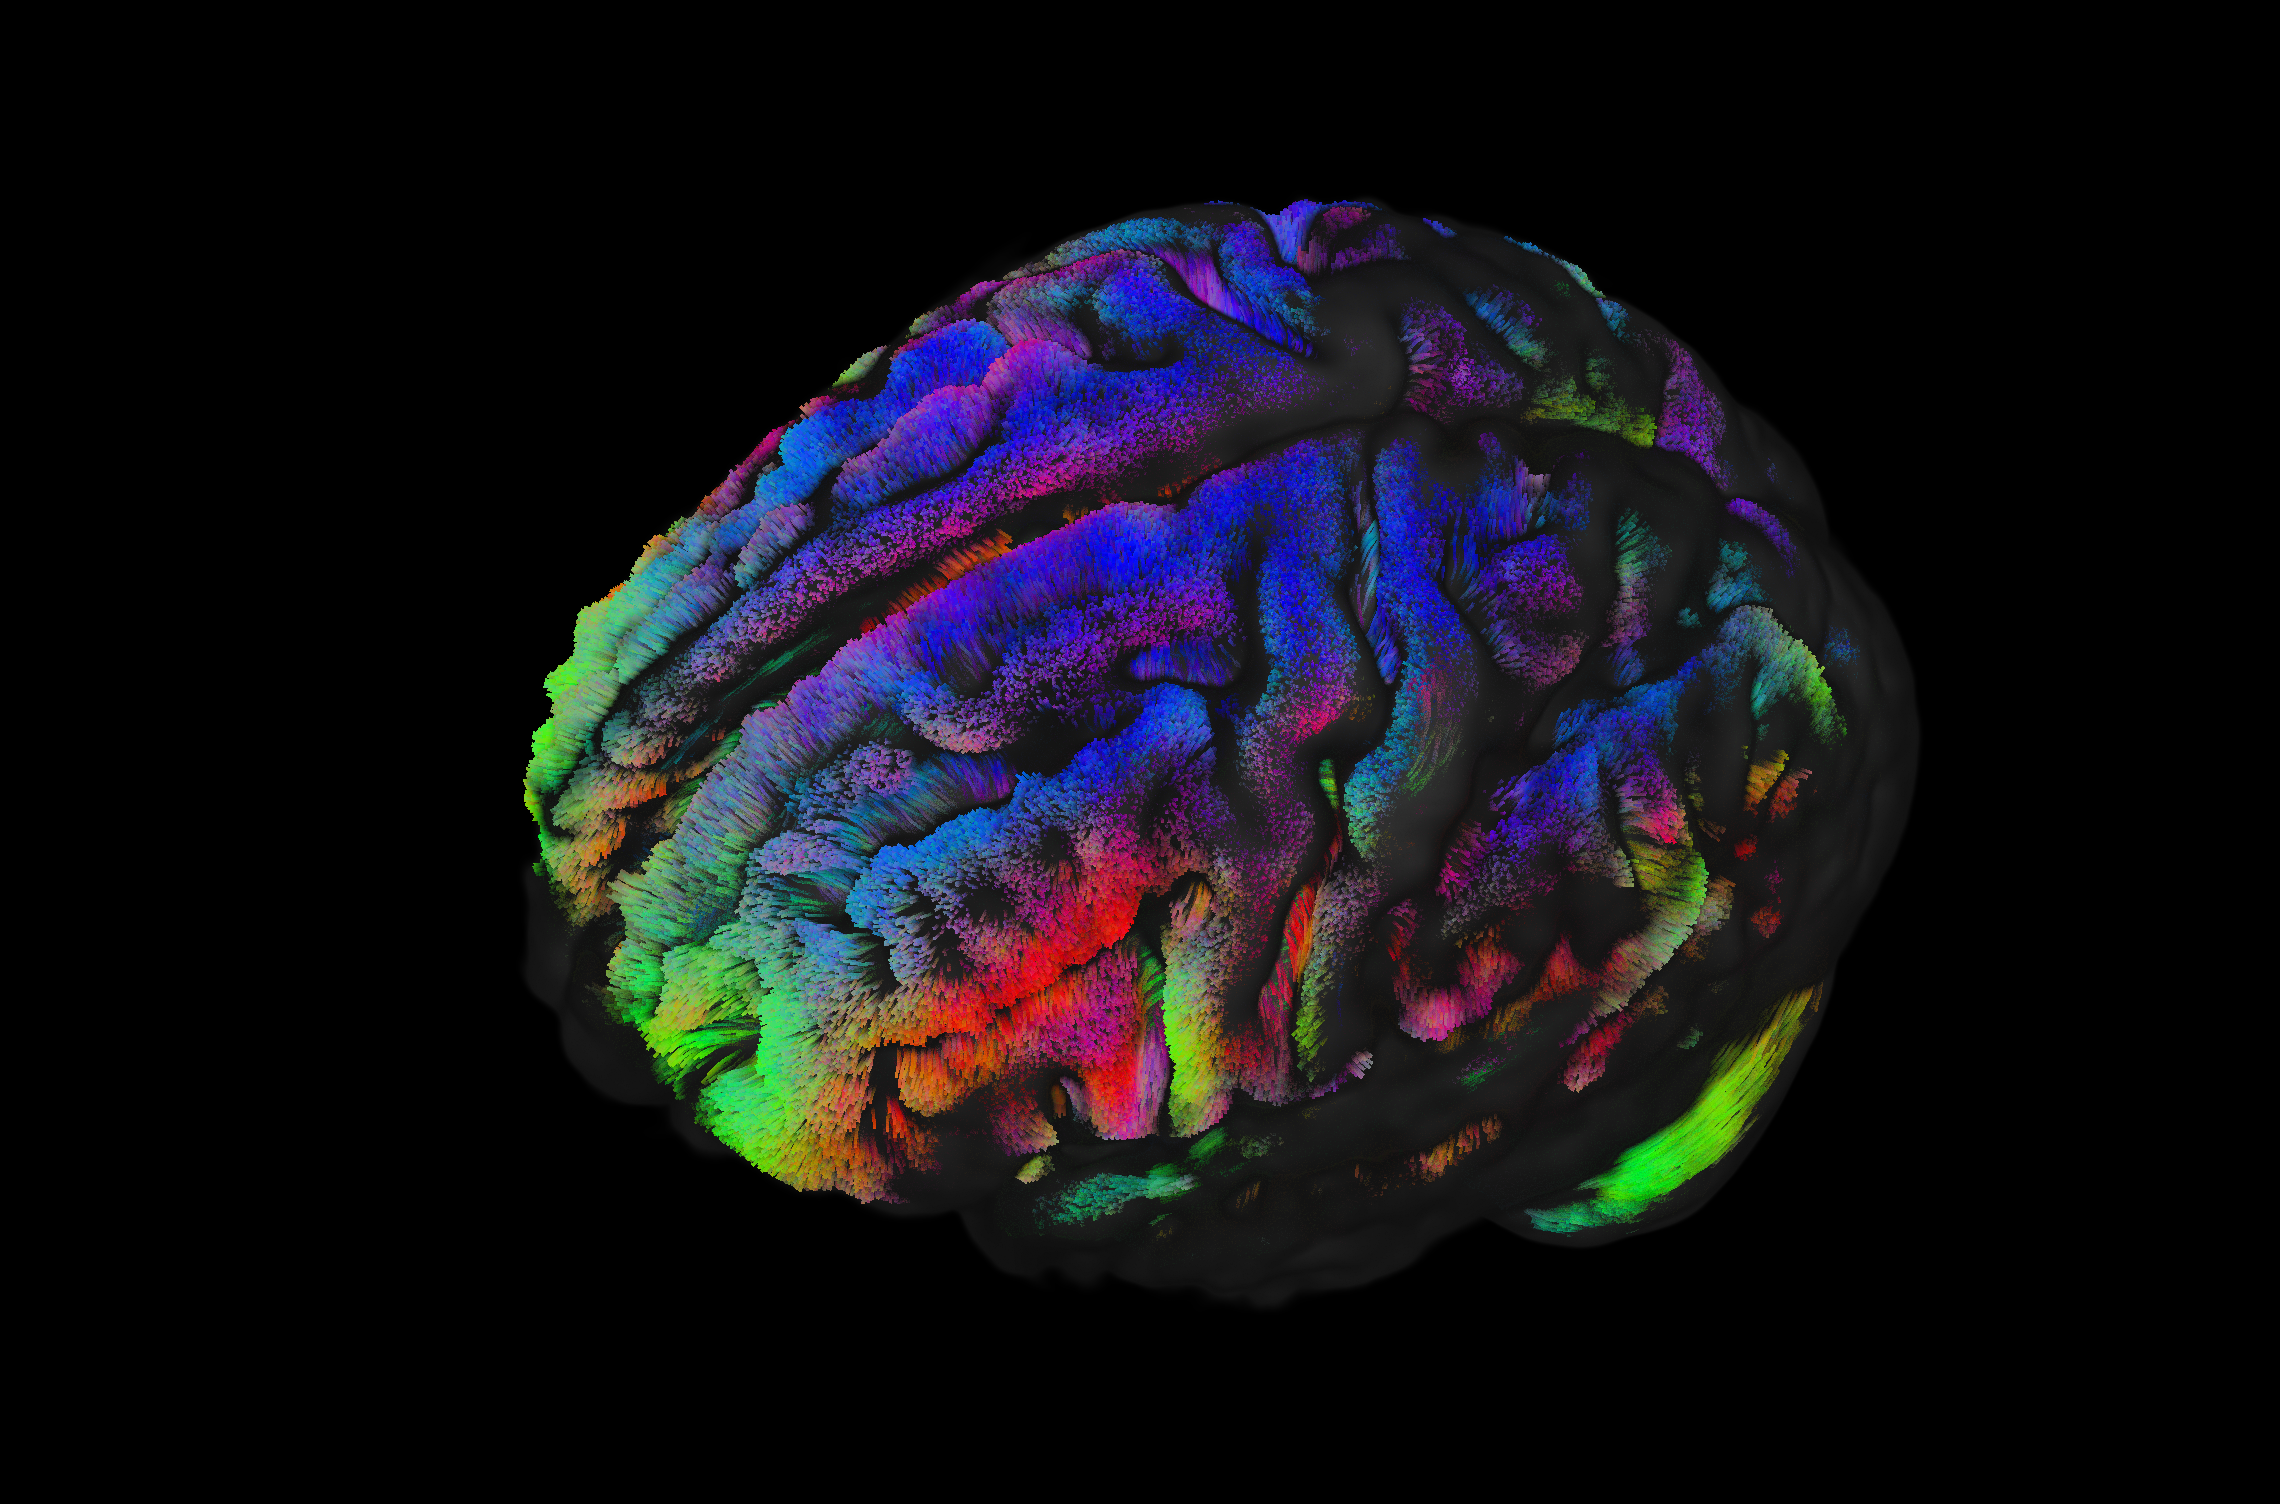
\includegraphics[width=0.5\textwidth]{Images/tractography.png} % or use height= for vertical sizing
  \caption{Tractography of the template obtained using the results of MT-CSD.}
  \label{fig:tractography}
\end{figure}

\section{Statistical Analysis}
For FBA, we can formulate the statistical analysis as a GLM which has the form \cite{Winkler2014}:
\begin{equation}
{Y} = {M} \boldsymbol{\psi} + \boldsymbol{\epsilon}
\end{equation}
where ${Y}$ is the observed data, ${M}$ the design matrix, $\boldsymbol{\psi}$ contains the regression coefficients estimated using least squares, and $\boldsymbol{\epsilon}$ the random errors.
We can split ${M}$ in the following way:
\begin{equation}
{Y} = {X} \boldsymbol{\beta} + {Z} \boldsymbol{\gamma} + \boldsymbol{\epsilon}
\end{equation}
where ${X}$ contains the regressors of interest and ${Z}$ the nuissance regressors (covariates).

In our case ${Y}$ is the values of a certain metric (e.g., AFD) for a specific fixel across all subject in the study. So, it will have dimension of 101x1. Since we want to compare the different groups, ${X}$ contains one column per group (CP, CM, HC), resulting in dimensions 101x3, with a 1 indicating group membership and 0 otherwise. ${Z}$ contains a column for the age and one for the intracranial volume (ICV) when relevant. ICV can play a role when analyzing FC and FDC, as they contain information regarding volume changes. Both age and ICV need to be normalized. In this model, the values of the vector $\boldsymbol{\beta}$ ($\beta_1$, $\beta_2$, $\beta_3$) represent the mean metric value for each group when the covariates are 0 (at mean age and ICV). The coefficients of $\boldsymbol{\gamma}$ reflect the effect of the covariates.

To formally test hypotheses about group differences, a contrast matrix $\mathbf{C}$ is defined. For a one-sided directional test, the null hypothesis is written as \cite{Winkler2014}:

\begin{equation}
H_0: {C}\boldsymbol{\psi} \leq 0
\end{equation}

${C}$ defines a linear combination of model parameters. In our case we are interested in testing differences in the mean values between groups. For example, ${C} = [-1 \; 0 \; 1 \; 0 \; 0]$ tests whether $\beta_3 > \beta_1$, i.e., whether the metric is higher in healthy controls (HC) than in chemo-treated patients (CP) for a given fixel. Since the interpretability of the fixel-wise metrics may not always be straightforward, both directions need to be tested (e.g., $\beta_3 > \beta_1$ and $\beta_1 > \beta_3$).
\\In the analysis,  the pairwise difference in both directions between groups for all metrics will be tested and significance will be determined as described in the previous chapter, using permutation testing and CFE.

\section{Statistical Power and Track Density Imaging}
Given the large number of fixels (on the order of 300,000), and so of statistical tests, corrections for multiple comparisons can become so stringent that detecting meaningful effects is extremely difficult. 
One common approach to partially solve this problem is to reduce the number of tests by focusing on specific regions of interest \cite{Cremers2017, Lindquist2015}. 
For example, prior knowledge about which brain regions are related to the disease of interest can guide the selection of relevant tracts, as demonstrated in the context of FBA by Mito et al.\ \cite{Mito2018}.
Another way to enhance statistical power, without the need to choose a region of interest (ROI) a priori, is through tract density imaging (TDI) \cite{Calamante2010}. This technique uses the results of tractography to generate an image in which voxel intensity reflects the number of streamlines passing through each voxel. This can be extended to fixels by assigning to each one the number of streamlines passing through it. Then, we can apply a threshold to generate a fixel mask, excluding from the analysis fixels with low streamline density, which are likely to be poorly connected to the rest of the brain. This allows to focus on more meaningful regions and improve the chances of detecting significant effects.